\chapter{Solution}

To achieve our objective, in this work we tried to focus on the day to day activities of the CHWs. The purpose is to analyze how they carrie out their activities, what information they get when treating their patients and how they link back time to time in the health care system.The figure below describes the current work flow of the CHWs.

\begin{figure}[H]
%\begin{center}
\centering
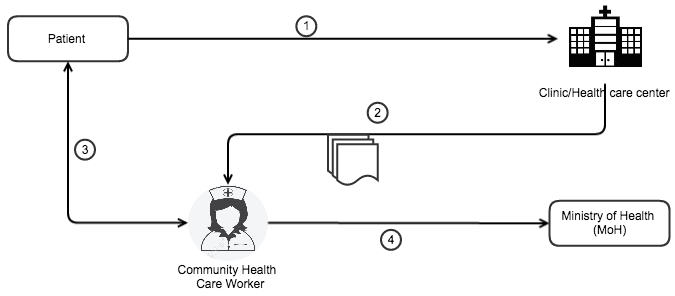
\includegraphics[width=10cm]{images/current_situation.png} % This scales the picture to
                                      % a width of 10cm
                                      % You can scale to the
                                      % width or height you need
%\end{center}
\caption{Current CHWs work flow}
\label{fig:fig-eg}  
\end{figure}

As the figure shows, the first step consist of a patient getting the first diagnosis by an actual clinician at the nearest clinic. The diagnosis information are then shared with the CHW living in the same or nearest vicinity with the patient. The figure also show how the information are shared only with the ministry of health in the form of reports. As mentioned above, this flow has improved the health condition of the citizens since there is that continuous and regular health service delivered by CHWs,  but there are still room to improve and make it more effective.

Before getting access to a particular doctor, more emerging diseases resistant to drugs due to rudimental health care practices and eventually deaths. In developing a solution for the outlined issues, an hypothesis was developed on how mobile technologies and health-care sensors can be combined to improve community health-care values. The application of internet of things in health-care have been trending around the world where we see a lot of solutions emerging trying to solve various issues. In Rwanda the Ministry of Health (MoH) and its partners have implemented different systems around health-care to support in the better management of activities around the country including few SMS applications such as the RAPID SMS platform that provide simple sms application functionalities that allows CHWs to conducts monitoring of women during their pregnancy, in the period of delivering and also for a short period of about one year after the baby was born. Currently in Rwanda there is no evidence of a developed project where health care sensors are used to collect different physiological data of a patient and share it in real time with a doctor for further analysis and decision making. the current existing methods patient are require to visit the doctors in order to know what it is going on in their health or CHWs use their ineffective tools that can measure some few vital signs with a huge margin of errors that can put the patient in danger and can result in bad treatment of certain diseases.

To measure our hypothesis, a one of a kind system is developed using IoT technologies. To have more impact on improving the health status of the community in rural areas, this system is developed to be used by CHWs in their every day activities. The developed solution in this work is to enhance the existing system by allowing bidirectional flow of information between CHWs and experienced medical workers. By using open source technology, the solution will solve the issue of lack of proper and accurate diagnostic tools by CHWs. The figure bellow shows how the solution will enhance the existing CHWs by allowing them to have access to more relevant tools and information to help them to make more important interventions and make quicker and effective decisions.

\begin{figure}[H]
%\begin{center}
\centering
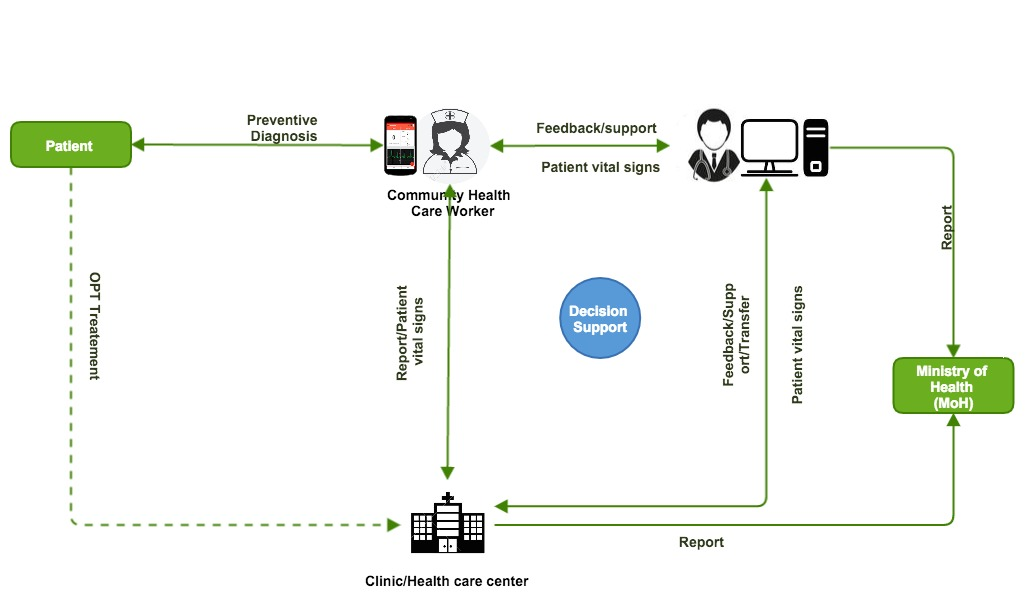
\includegraphics[width=15cm]{proposed_solution.jpg} % This scales the picture to
                                      % a width of 10cm
                                      % You can scale to the
                                      % width or height you need
%\end{center}
\caption{New proposed CHWs work flow}
\label{fig:fig-eg}  
\end{figure}
